% !TEX spellcheck = uk_en
\documentclass[main.tex]{subfiles} 

\begin{document}

\section*{Undervisningsopplegget}
\label{sec:1}

Vi, lærerstudentene, observerte elevene fra 8. klasse i både naturfagtimer og matematikk timer. 
Elevenes faglig bakgrunn er varierende, klassen har en gjennomsninttelig fordeling av fagelig 
sterke og faglig svake elever. Før undervisningsopplegget ble utført observerte vi elevene 
gjennom flere timer, blant annet i en naturfag time. I denne timen brukte elevene mikroskop 
for å studere diverse celleprøver, blant annet fra deres egen munn. Timen startet med 
repitisjon av begreper om celler og mikroskop. Elevene ble fordelt i grupper på 3-4 stykker, 
og læreren gikk rundt og veiledet alle gruppene, deriblant hjalp læreren med å innstille 
mikroskopene til elevene slik at de endte opp med riktig fokus. Læreren gjennomgikk deretter 
felles med elevene med et mikroskop som var koblet til en datamaskin. Bildet fra mikroskopet 
ble projisjert på lystavlen i laboratoriet. Dette inspirerte oss til å bruke en tilsvarende 
opplegg til å strukturere vår egen undervisningstime(r), og faller under det John Dewey (1859 - 
1952) kaller utforskende arbeidsmåter, \citeA{rogs13}, \citeA[kap. 1]{knai11}.

Undervisningssekvesene vi har forberedt har til hensikt å utfylle følgende \textbf{kompetansemål 
i læreplanen}
\newline
\newline
\emph{Forskerspiren} :
\begin{itemize}
\vspace{-2mm}
\item formulere testbare hypoteser, planlegge og gjennomføre undersøkelser 
av dem og diskutere observasjoner og resultater i en rapport
\end{itemize}
\emph{Mangfold i naturen} :
\begin{itemize}
\vspace{-2mm}
\item beskrive oppbygningen av dyre- og planteceller og forklare hovedtrekkene i fotosyntese 
og celleånding
\vspace{-5mm}
\item gjøre rede for celledeling og for genetisk variasjon og arv
\end{itemize}
Undervisningseksvensene er fordelt over 3 skoletimer over 2 uker. Opplegget ble laget i henhold
til forutsetningene til elevene og deres bakgrunn basert på våre observasjoner og 
tilbakemeldinger fra veileder. Dette opplegget utførte jeg alene, med veileder og en medstudent 
som observatører. De bidro også i blant med å gi personlig/gruppe veiledning når elevene jobbet
enten selvstendig eller sammen i grupper.

\subsection*{Microsoft OneNote}

I undervisningen ble OneNote brukt til de første to timene. OneNote er en dataprogram som lar 
brukere inntaste enten fra tastatur, eller kan anvendes sammen med en smartboard med en stylus til å
føre håndskrevne notater. Bilder, tabeller og videor kan settes inn i notatene. Sidene i notatene 
blir lagret automatisk og organisert i seksjoner i notatboken. Isteden for tavleundervisning, 
ble OneNote brukt til å føre forelesningsnotater, og i et av sekvensene ble 
digitalerepresentasjoner brukt til å fremstille organsystemer (se figurene \ref{fig:notat1} -
\ref{fig:notat2}). Disse notatene blir lagret på nettskyen, som elevene kan ha lesetilgang til
fra sine private koblinger. Elevene har ikke tilgang til egne maskiner i timene (siden dette 
strider mot skolens ordensregler om bruk av mobiler og andre verktøy i timen), med mindre en 
så-kalt laptoptralle blir hentet til klassen av underviseren. En slik tralle inneholder flere 
pcer som elevene låner midlertidig for å utføre skolearbeid. I våre timer valgte vi å ikke 
benytte laptoptrallen siden undervisningen ble ført på lystavlen og elevene ble isteden bedt 
om å ta skriftlige notater. Noe som viser seg ikke er normen, med mindre elevene blir 
eksplisitt bedt om å ta notater. Dette vil vi senere gå nærmere inn på når vi analyserer 
undervisningssekvensene.

\begin{figure}[h!]
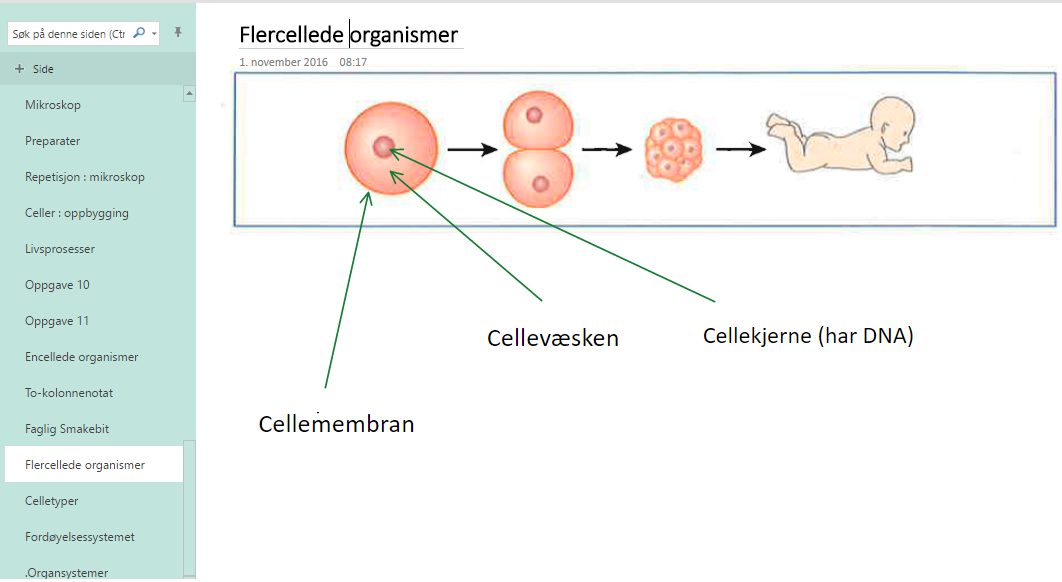
\includegraphics[scale = 0.6]{../figures/onenote_flercellet.png}
\caption{notat 1}
\label{fig:notat1}
\end{figure}

\begin{figure}[h!]
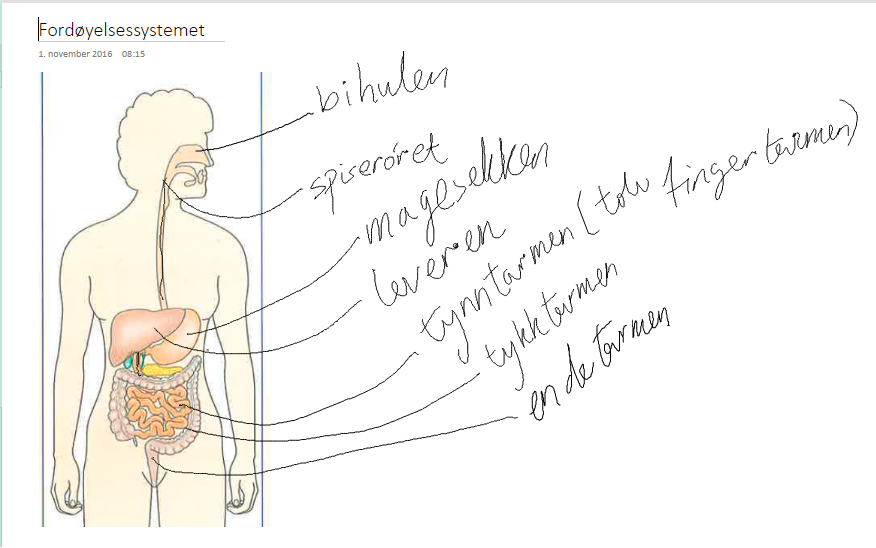
\includegraphics[scale = 0.6]{../figures/onenote_fordoyelse.png}
\caption{notat 2}
\label{fig:notat2}
\end{figure}

\subsection*{1. time}

Hensikten med denne timen er å oppsumere det elevene har lært hittil om celler og 
levendeorganismer, og innføre et nytt tema om encellede organismer. Timen starter med repetisjon 
av det elevene har lært fra tidligere timer, deriblant om mikroskop og cellestrukturen. Ved oppstart 
av timen initierer vi elevene til å reflektere over temaer og begreper de har lært -og hatt lekser 
om. Vi bruker IRE/F metoden, der vi spørr elevene som rekker opp hånda. Det viser seg at det 
er noen få elever, som viser trygghet og kontroll når de responderer til lærer initiert dialog. 

En av de viktigste egenskapene en lærer kan utvise er evnen til å tilpasse seg i forhold til 
klassen, en gruppe eller på individ nivå. Ved å erkjenne at alle elevene skal ha kjennskap til 
begrepene som blir tatt opp og repetert, er det da nødvendig å få bekreftet at elevene innehar en 
overordnet forståelse. Det kan derfor være nødvendig å frempeke noen elever som ikke viser aktiv 
deltagelse i timen og frembringe deres respons. Derimot er dette problematisk hvis det viser seg at 
de ikke har forutsetninger til å kunne respondere. Da settes de i en vanskelig situasjon hvor det 
blir nødvendig for læreren å lede de ut, ved hjelp av for eksempel ledende spørsmål. Derimot hvis 
det er forventet at det er en del av forutsetningene at elevene skal kunne respondere til lærer 
initiativ, da kan utspørringen av elevene vise hull i deres kunnskap. I neste time blir en 
annen form for lærer initiativ brukt til å frembringe respons. 
 
Siden elevene gjennom heleklassesamtalen har blitt "varmet" opp kognitivt, er de mottagelige for å 
lære om et nytt tema. Innføringen av nytt tema er bevisst satt opp på en slik måte at overgangen 
fra repetisjon til det nye temaet blir naturlig og flyttende. Hensikten er å la elevene danne et 
helhetlig bilde om celler. I timene hvor de har hatt en innføring om celler, har de lært om basale 
strukturer. I denne timen går de litt dypere ved å få en innføring om en av klassifikasjonene av celler.
Hensikten med innføringen er todelt : gjøre elevene bevisst om at det finnes forskjellige type
celler, og gjøre de klar for den siste timen hvor de vil studere slike type celler under mikroskop.

Siden det er til hensikt å bruke resterende del av timen til repetisjon, er det ikke nødvendig å 
prøve å finne svakheter i elevenes respons gjennom helklassesamtalen. For å finne slike svakheter 
ble gruppesamtalene en bedre plattform. I den forbindelse ble tokolonnenotatet tatt i bruk (se 
vedlegg : \ref{sec:tokolonnenotat}). Hensikten med denne øvelsen er å la elevene jobbe sammen
i grupper om samme tema, hvor de blir enige med hverandre om hva som er viktig å være klar over. 
Deretter fordeles de i nye grupper slik at hver gruppe har minst en elev som har forbredt sitt sett 
med temaer/begreper. Under hele denne prosessen er vi tilgjengelige til å gå rundt og høre elevene 
diskutere begreper, først sammen i grupper, og deretter individuelt når de fremfører sine 
konklusjoner med medelever. Hvis vi merker at eleven har problemmer med å gi tilstrekkelig 
respons om en gitt tema, initierer vi eleven i en dialog hvor vi forsøker å konstruere sammen en 
mer utdypet forståelse om begrepene. 

\subsection*{2.time}

Timen starter på tilsvarende vis som den første timen. Derimot i denne timen er oppsettet 
forskjellig. Hensikten med timen er å repetere leksene elevene har fått til timen, om celletyper og
utvikling av celler fra enkeltceller til flercelledeorganismer. Etter å konsultert med vår veileder 
var vi nå klar over at alle elevene hadde forutsetning til å kunne respondere til våre spørsmål, 
så lenge de var relatert til leksene. Etter den første timen var vi nå bevisste på at elevenes 
respons var avhengig av deres trygghet med et gitt tema. Vi valgte derfor å bruke navnekort 
isteden, hvor en elevs' navn ble opplest vilkårlig fra en usortert liste, og deretter fikk eleven 
ordet og tid til å respondere. Elev respons ble enten akseptert, eller hvis eleven viste svakheter
i sin forståelse ble spørsmålet gitt til andre i klassen og dialogen ble avsluttet med en vurdering,
og hvis nødvendig tilleggsinformasjon ble supplert. 

Hensikten med repetisjonen er å frembringe og forsterke prosessen for en flercellet organisme fra 
en enkelt celle (se \ref{fig:notat1}). For å få til dette begynte vi timen med å starte med en 
enkelt celle, videre til å skille mellom forskjellige typer celler og hvordan de er med å danne 
vev, og prosessen fra vev til organer, og fra organer til organssystemer. Når vi begynte å snakke
om organsystemer benyttet vi oss av en anatomisk modell av overkroppen. Vi brukte den til å snakke 
om fordøyelsessystemet.
Den anatomiske modellen består av organer som er avtagbare (nesten som legoklosser) og flere organer 
kan dermed ses, som ligger i bakgrunnen. Gjennom hele forklaringen om fordøyelsessystemet benyttet 
vi elevene som ble stilt kontrollspørsmål underveis. De bidro med å gi en forklaring for hele prosessen, 
fra maten blir tygd, til at den blir brutt ned i tarmene og næringen blir tatt opp gjennom blodstrømmen, 
og tilslutt avfall som blir utskilt fra endetarmen. Vi gjentok denne prosessen på OneNote (se 
\ref{fig:notat2}). Etter at alle temaene hadde blitt gjennomgått, begynte vi den samme prosessen, 
men med omvendt rekkefølge, med hensikt å vise at mennesker består av milliarder av celler og 
at vi kan spore vår oppvekst tilbake til befruktningsprosessen, hvor vår opphav er nemlig som
encellede organismer. Ved å bruke denne fremgangsmåte merket vi at konseptene ble grundigere
gjennomgått og rekkefølgen virket logisk og oversiktelig. Gjentagelsen av rekkefølgen i motsatt
rekkefølge ble brukt til å forsterke elevenes forståelse for begrepene og danne en logisk 
rekkefølge i deres tankebaner. Etter at vi ble ferdige lot vi noen av elevene sette sammen
den anatomiske modellen. Vår veileder benyttet denne anledningen til å undersøke om noen
av elevene hadde gjort sine lekser ved å se på deres notatbøker.

\subsection*{3.time}
Opprinnelig hadde vi planlagt å utføre innhenting av nødvendig materialer for å gjennomføre 
mikroskop øvelsen ved å få elevene til å utføre innsamlingen gjennom en skoleutflukt. Utflukten var 
en del av valgfaget friluftsliv. Fra vår klasse var det 7 elever som deltok i utflukten. Vår hensikt
var opprinnelig å få disse elvene til å samle inn døde planter og vann. Derimot endte vi (dvs. 
lærerstudentene) med å gjøre innsamlingen selv grunnet sen planlegging av timen. 

Når denne siste timen startet hadde vi allerede bevart prøvene fra utflukten en uke i laboratoriet. 
Gjennom tilstrekkelige forhold hadde vi klart å vokse fram encellede organismer, deriblant tøffeldyr 
(en organisme som er oppkalt etter sko grunnet at dens utseende ligner på tøfler).

Timen ble utført i laboratoriet i skolen. Vi startet timen ved å bruke tavlen hvor vi førte opp
hensikten og målet med timen. Deretter informerte vi elevene om hvordan prøvene ble innsamlet
og hvordan de skal studeres under et mikroskop. Etter at vi hadde formidlet informasjonen både
muntlig og skriftlig (på tavlen) ba vi elevene om å lese om øvelsen fra deres lærebok. Deretter
fordelte vi elevene i grupper og vi delte roller til alle i gruppene. Noen i gruppene hentet
mikroskop og innstilte den, mens andre hentet utstyr som objektivglass, vannprøver og bomull.
Etter at elevene hadde samlet utstyr og var klare til å studere prøvene, informerte vi elvene
om hvordan de kan bruke bomull til å absorbere vannprøvene og studere organismene under mikroskopet.
Siden elevene hadde brukt mikroskopene fra en tidligere laboratorieøvelse, ble de bedt om å 
gjennomføre resten av forsøket på egenhånd. Etter at vi hadde delt ut alle instruksene gikk vi
rundt og observerte elevene. En del av gruppene hadde problemmer med for eksempel overbruk av bomull, 
eller så tilsatte de for lite vann på objektetglasset. Noen av gruppene fikk hjelp med å finne 
riktig innstillinger for å studere organismene. Samtidig forberedet vi vår egen prøve i mikroskopet 
som var koblet til en datamaskin. Etter at vi hadde observert at alle elevgruppene hadde klart å 
observere mikro organismene og deres oppførsel, utførte vi eksperimentet på vår egen mikroskop.
Deretter instruerte vi elvene til å studere en annen prøve som innsamlet fra en forskjellig kilde.
Elevene gjentok forsøket og gjorde sine observasjoner. Tilslutt gikk vi gjennom hva de forskjellige
gruppene observerte og intruerte elevene til å lage en rapport som skal leveres inn på It's Learning.
Siden dette var første gangen de har blitt bedt om å lage en rapport i naturfagtimen informerte vi 
elevene om hva vi forventet skal stå i rapporten.

\end{document}